\begin{frame}{Object Storage (1): Object overview}
  \begin{itemize}
    \item git is a key-value store
    \begin{itemize}
      \item keys = SHA-1 hashes
    \end{itemize}
    \item Three main types of objects:
    \begin{itemize}
      \item BLOBs (for file content)
      \item Trees (for storing a directory of files)
      \item Commits (to store multiple versions)
    \end{itemize}
  \end{itemize}
\end{frame}

\begin{frame}[fragile]{Object Storage (2): BLOBs}
  \begin{itemize}
    \item stores the \textit{content} of a file
    \item problem: no meta-information such as filename, path
  \end{itemize}
\begin{lstlisting}[style=ShellCmd]
$ echo 'test content' | git hash-object -w --stdin
d670460b4b4aece5915caf5c68d12f560a9fe3e4
\end{lstlisting}
\begin{lstlisting}[style=ShellCmd]
$ git cat-file -p d670460b4b4aece5915caf5c68d12f560a9fe3e4
test content
\end{lstlisting}
\begin{itemize}
  \item storing multiple versions of the same file is no problem
\end{itemize}

\begin{lstlisting}[style=ShellCmd]
$ echo 'version 1' > test.txt
$ git hash-object -w test.txt
83baae61804e65cc73a7201a7252750c76066a30
\end{lstlisting}

\begin{lstlisting}[style=ShellCmd]
$ echo 'version 2' > test.txt
$ git hash-object -w test.txt
1f7a7a472abf3dd9643fd615f6da379c4acb3e3a
\end{lstlisting}

\end{frame}

\begin{frame}[fragile]{Object Storage (3): BLOBs continued}
  \begin{itemize}
    \item we can checkout each version individually
  \end{itemize}
\begin{lstlisting}[style=ShellCmd]
$ git cat-file -p 83baae61804e65cc73a7201a7252750c76066a30 > test.txt
$ cat test.txt
version 1
\end{lstlisting}

\begin{lstlisting}[style=ShellCmd]
$ git cat-file -p 1f7a7a472abf3dd9643fd615f6da379c4acb3e3a > test.txt
$ cat test.txt
version 2
\end{lstlisting}

\begin{itemize}
  \item the objects are just stored on disk
\end{itemize}

\begin{lstlisting}[style=ShellCmd]
$ find .git/objects -type f
.git/objects/d6/70460b4b4aece5915caf5c68d12f560a9fe3e4
.git/objects/83/baae61804e65cc73a7201a7252750c76066a30
.git/objects/1f/7a7a472abf3dd9643fd615f6da379c4acb3e3a
\end{lstlisting}

\begin{itemize}
  \item their type is also stored
\end{itemize}

\begin{lstlisting}[style=ShellCmd]
$ git cat-file -t 1f7a7a472abf3dd9643fd615f6da379c4acb3e3a
blob
\end{lstlisting}

\end{frame}

\begin{frame}[fragile]{Object Storage (4): Trees}
  \begin{itemize}
    \item each node represents a single directory
    \item must contain 1 or more entries (so no empty folders)
    \item includes file names + mode
  \end{itemize}
\begin{lstlisting}[style=ShellCmd]
$ git cat-file -p master^{tree}
100644 blob a906cb2a4a904a152e80877d4088654daad0c859      README
100644 blob 8f94139338f9404f26296befa88755fc2598c289      Rakefile
040000 tree 99f1a6d12cb4b6f19c8655fca46c3ecf317074e0      lib
\end{lstlisting}
\begin{lstlisting}[style=ShellCmd]
$ git cat-file -p 99f1a6d12cb4b6f19c8655fca46c3ecf317074e0
100644 blob 47c6340d6459e05787f644c2447d2595f5d3a54b      simplegit.rb
\end{lstlisting}
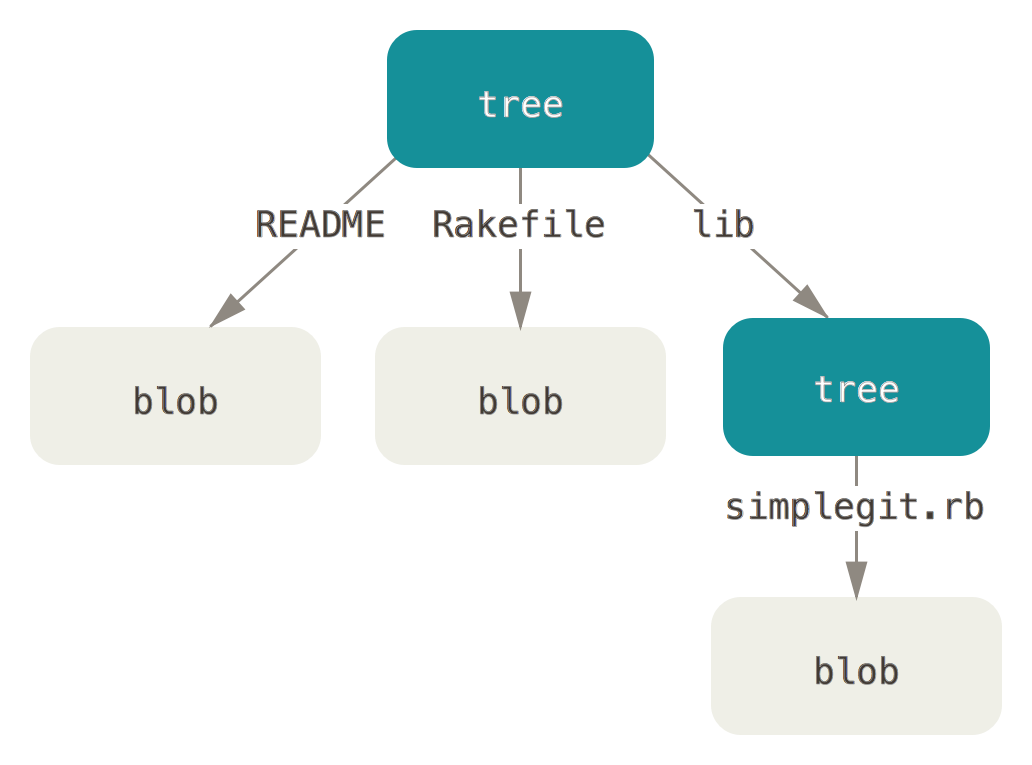
\includegraphics[width=0.60\textwidth]{imgs/object_tree}
\end{frame}

\begin{frame}[fragile]{Object Storage (5): The Index as a Tree}
  \begin{itemize}
    \item we can use a tree to represent the index
    \item we can update the tree with the file we created above
  \end{itemize}
\begin{lstlisting}[style=ShellCmd]
$ git update-index --add --cacheinfo 100644 \
  83baae61804e65cc73a7201a7252750c76066a30 test.txt
$ git write-tree
d8329fc1cc938780ffdd9f94e0d364e0ea74f579
$ git cat-file -p d8329fc1cc938780ffdd9f94e0d364e0ea74f579
100644 blob 83baae61804e65cc73a7201a7252750c76066a30      test.txt
\end{lstlisting}

  \begin{itemize}
    \item we can add yet another file to it
  \end{itemize}

\begin{lstlisting}[style=ShellCmd]
$ echo 'new file' > new.txt
$ git update-index test.txt
$ git update-index --add new.txt
$ git write-tree
0155eb4229851634a0f03eb265b69f5a2d56f341
\end{lstlisting}
\end{frame}

\begin{frame}[fragile]{Object Storage (6): The Index as a Tree continued}

  \begin{itemize}
    \item we can also add the same tree as a sub-directory
  \end{itemize}

\begin{lstlisting}[style=ShellCmd]
$ git read-tree --prefix=bak d8329fc1cc938780ffdd9f94e0d364e0ea74f579
$ git write-tree
3c4e9cd789d88d8d89c1073707c3585e41b0e614
$ git cat-file -p 3c4e9cd789d88d8d89c1073707c3585e41b0e614
040000 tree d8329fc1cc938780ffdd9f94e0d364e0ea74f579      bak
100644 blob fa49b077972391ad58037050f2a75f74e3671e92      new.txt
100644 blob 1f7a7a472abf3dd9643fd615f6da379c4acb3e3a      test.txt
\end{lstlisting}

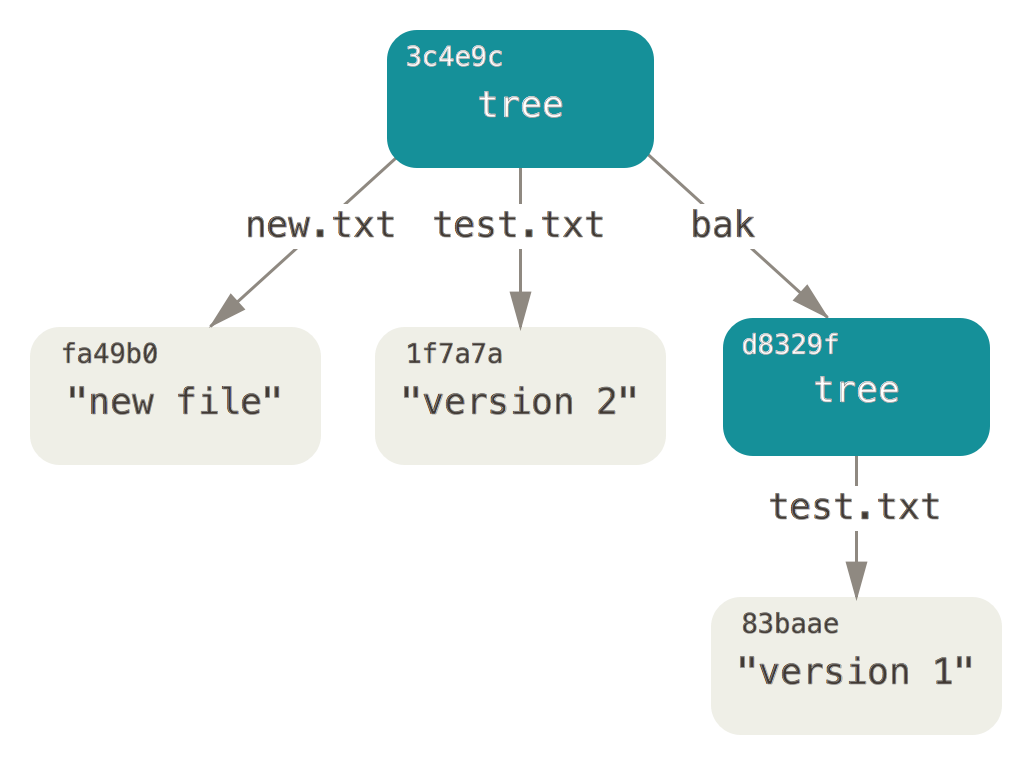
\includegraphics[width=0.60\textwidth]{imgs/index_tree}
\end{frame}

\begin{frame}[fragile]{Object Storage (7): Commit objects}

  \begin{itemize}
    \item we also want to store different commits
    \item each commit contains
    \begin{itemize}
      \item a tree representing the current state
      \item the parent commit
      \item meta-information, such as author and time
      \item (you may get different SHAs because of this)
    \end{itemize}
  \end{itemize}

  \begin{itemize}
    \item we can make a single commit
  \end{itemize}
  
\begin{lstlisting}[style=ShellCmd]
$ echo 'first commit' | git commit-tree d8329f
35f8b9255a9c68f80d90201ae14c39d9c9b66b2a
$ git cat-file -p 35f8b9
tree d8329fc1cc938780ffdd9f94e0d364e0ea74f579
author Tom Wiesing <tkw01536@gmail.com> 1458923656 +0100
committer Tom Wiesing <tkw01536@gmail.com> 1458923656 +0100

first commit
\end{lstlisting}

\begin{itemize}
  \item we can also make commits referencing earlier ones
\end{itemize}

\begin{lstlisting}[style=ShellCmd]
$ echo 'second commit' | git commit-tree 0155eb -p 35f8b9
0d9d54e2c438e22d6656fa1bdca7d76a36d3589c
$ echo 'third commit'  | git commit-tree 3c4e9c -p 0d9d54
970ac2c0207ad51caccce0a71d21283ff7109254
\end{lstlisting}
\end{frame}

\begin{frame}[fragile]{Object Storage (8): Commit objects continued}
  \begin{itemize}
    \item we can now look at the history
  \end{itemize}
\begin{lstlisting}[style=ShellCmd]
$ git log --stat 970ac2
commit 970ac2c0207ad51caccce0a71d21283ff7109254
Author: Tom Wiesing <tkw01536@gmail.com>
Date:   Fri Mar 25 17:38:21 2016 +0100

    third commit

 bak/test.txt | 1 +
 1 file changed, 1 insertion(+)

commit 0d9d54e2c438e22d6656fa1bdca7d76a36d3589c
Author: Tom Wiesing <tkw01536@gmail.com>
Date:   Fri Mar 25 17:38:07 2016 +0100

    second commit

 new.txt  | 1 +
 test.txt | 2 +-
 2 files changed, 2 insertions(+), 1 deletion(-)

commit 35f8b9255a9c68f80d90201ae14c39d9c9b66b2a
Author: Tom Wiesing <tkw01536@gmail.com>
Date:   Fri Mar 25 17:34:16 2016 +0100

    first commit

 test.txt | 1 +
 1 file changed, 1 insertion(+)
\end{lstlisting}
\end{frame}

\begin{frame}[fragile]{Object Storage (9): Commit objects continued}
  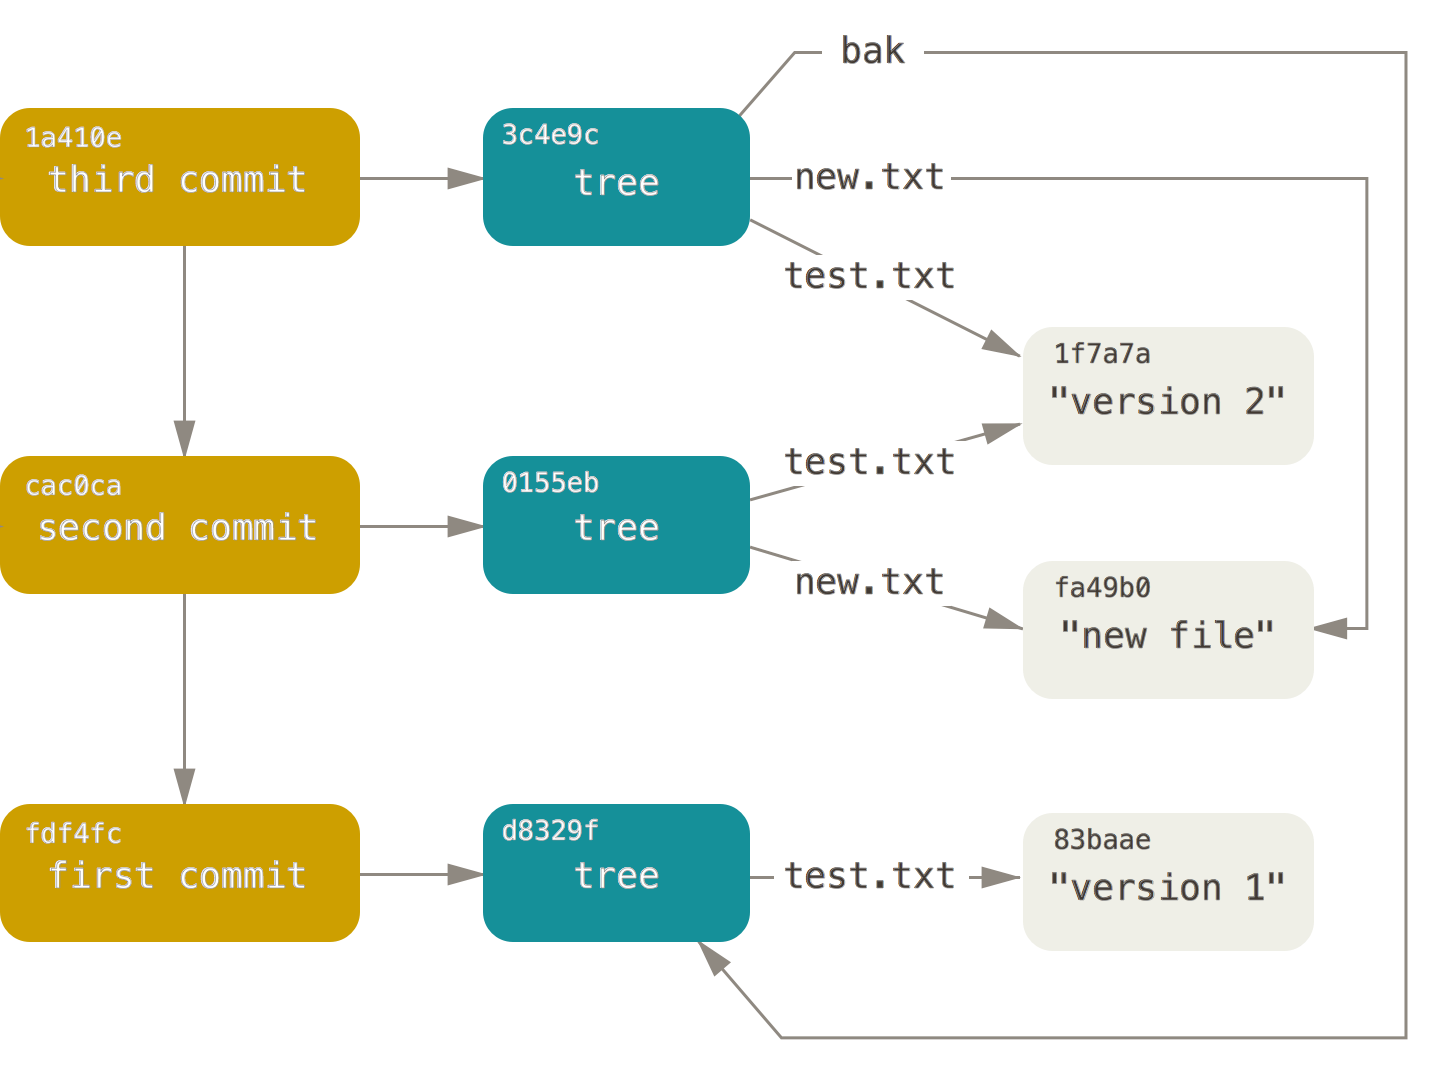
\includegraphics[width=0.90\textwidth]{imgs/commit_tree}
\end{frame}